\documentclass{beamer}

\usepackage{amsmath,amssymb}
\usepackage{tikz}
\usetikzlibrary{arrows,decorations,decorations.markings}

%
% Custom theme
%
\usetheme{AAUsimple}

%
% Custom operator declarations
%
\DeclareMathOperator{\ZZ}{\mathbb{Z}}
\DeclareMathOperator{\CC}{\mathbb{C}}
\DeclareMathOperator{\hh}{\mathfrak{h}}
\DeclareMathOperator{\re}{\text{Re}}
\DeclareMathOperator{\im}{\text{Im}}
\newcommand{\thetachar}[2] {\theta {\scriptsize \begin{bmatrix}#1\\#2\end{bmatrix}}}
\newcommand{\thetacharsm}[2] {\theta \left[ \begin{smallmatrix} #1
      \\ #2 \end{smallmatrix} \right]}

%%%%%%%%%%%%%%%%%%%%%%%%%%%%%%%%%%%%%%%%%%%%%%%%%%%%%%%%%%%%%%%%%%%%%%%%%%%%%%%
\title{Computational Applications of Riemann Surfaces and Abelian Functions}

\subtitle{General Examination}

\author{
  Chris Swierczewski\\
  {\tt cswiercz@uw.edu}
}

\institute{
  Department of Applied Mathematics\\
  University of Washington\\
  Seattle, Washington
}

\pgfdeclareimage[height=1.5cm]{titlepagelogo}{AAUgraphics/aau_logo_new_circle}

\titlegraphic{
  \pgfuseimage{titlepagelogo}
}

\AtBeginSection[]{\begin{frame}\frametitle{Goal of This Talk}\tableofcontents[currentsection,subsectionstyle=show/show/shaded]\end{frame}}
%%%%%%%%%%%%%%%%%%%%%%%%%%%%%%%%%%%%%%%%%%%%%%%%%%%%%%%%%%%%%%%%%%%%%%%%%%%%%%%



%%%%%%%%%%%%%%%%%%%%%%%%%%%%%%%%%%%%%%%%%%%%%%%%%%%%%%%%%%%%%%%%%%%%%%%%%%%%%%%
\begin{document}
%%%%%%%%%%%%%%%%%%%%%%%%%%%%%%%%%%%%%%%%%%%%%%%%%%%%%%%%%%%%%%%%%%%%%%%%%%%%%%%



\begin{frame}[plain,noframenumbering]
  \titlepage
\end{frame}



%%%%%%%%%%%%%%%%%%%%%%%%%%%%%%%%%%%%%%%%%%%%%%%%%%%%%%%%%%%%%%%%%%%%%%%%%%%%%%%
%\section*{Introduction}
%%%%%%%%%%%%%%%%%%%%%%%%%%%%%%%%%%%%%%%%%%%%%%%%%%%%%%%%%%%%%%%%%%%%%%%%%%%%%%%

%------------------------------------------------------------------------------
%\subsection*{Shallow Water Waves}
%------------------------------------------------------------------------------


\begin{frame}{Acknowledgments}{}
  \begin{itemize}
    \item Committee:
      \begin{itemize}
          \item Bernard Deconinck (advisor),
          \item Randy Leveque,
          \item Bob O'Malley,
          \item William Stein,
          \item Rekha Thomas (GSR).
      \end{itemize}
    \item Research Group:
      \begin{itemize}
        \item Olga Trichthenko,
        \item Natalie Sheils,
        \item Ben Segal.
      \end{itemize}
    \item Bernd Sturmfels (UC Berkeley),
    \item Jonathan Hauenstein (NCSU),
    \item Daniel Shapero (UW),
    \item Grady Williams (UW),
    \item Megan Karalus.
  \end{itemize}
\end{frame}



\begin{frame}{The Kadomtsev--Petviashvili Equation}{}
  \vspace{10pt}
  $u(x,y,t) = $ surface height of a 2D periodic shallow water wave.
  \[
  \tfrac{3}{4} u_{yy} = \frac{\partial}{\partial x} \left(
  u_t - \tfrac{1}{4} \left(6uu_x + u_{xxx}\right) \right)
  \]

  \begin{columns}[T]
    \begin{column}{0.5\textwidth}
      \begin{figure}
        \centering
        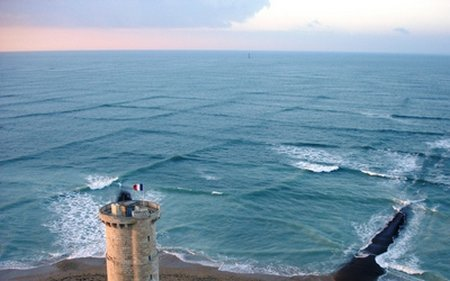
\includegraphics[width=\textwidth]{images/livekp.jpg}
        \caption{\^{I}le de R\'{e}, France}
      \end{figure}
    \end{column}
    \begin{column}{0.5\textwidth}
      \begin{figure}
        \centering
        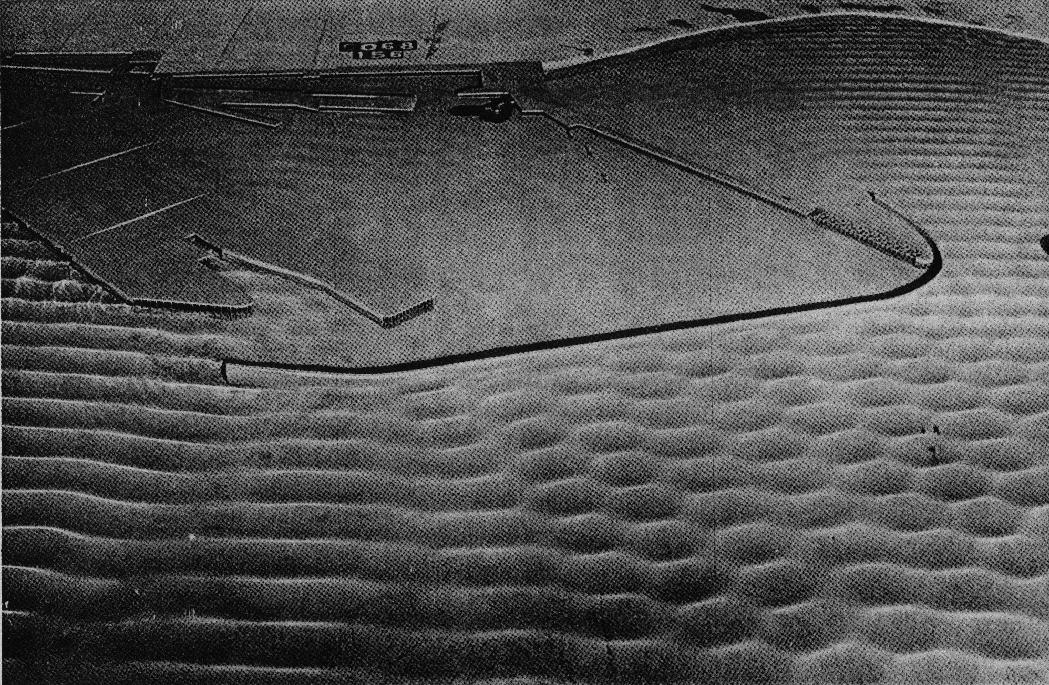
\includegraphics[width=\textwidth]{images/sd-harbor-model.jpg}
        \caption{Model of San Diego Bay}
      \end{figure}
    \end{column}
  \end{columns}
\end{frame}



\begin{frame}{Theta Function Solutions}{}
  Family of solutions: $\forall g \in \ZZ_+$
  \[
  u(x,y,t) = 2 \partial_x^2 \log
  \theta(Ux + Vy + Wt + z_0, \Omega) + c,
  \]
  \begin{itemize}
    \item $c \in \CC$,
    \item $U,V,W,z_0 \in \CC^g$,
    \item $\Omega \in \CC^{g \times g}$.
    \item {\it``Riemann theta function''} $\theta : \CC^g \times \CC^{g
      \times g} \to \CC$
  \end{itemize}

  \vspace{16pt}

  {\it Finite genus solutions}:
  \begin{itemize}
    \item dense in space of periodic solutions to KP.
  \end{itemize}
\end{frame}



\begin{frame}{The Riemann Theta Function}
  \[
    \theta(z,\Omega)
    =
    \sum_{n \in \ZZ^g}
    e^{
      2 \pi i
      \left( \tfrac{1}{2} n \cdot \Omega n + n \cdot z \right)
    }
  \]

  \uncover<2>{
  \begin{block}{\bf Convergence}
    \begin{itemize}
      \item Requires $\im(\Omega) > 0$.
      \item Also need only consider $\Omega^T = \Omega$.
      \item Space of {\it Riemann matrices}:
      \[
          \hh_g = \big\{ \Omega \in \CC^{g \times g} \; | \;
                     \Omega^T = \Omega \text{ and } \im(\Omega) > 0 \big\}
      \]
      (Siegel upper half space.)
      \[
          \theta:\CC^g \times \hh_g \to \CC
      \]
    \end{itemize}
  \end{block}
  }
\end{frame}

\begin{frame}{Abelian Functions}{}
  Periodic, meromorphic functions
  \[
      f : \CC^g \to \CC
  \]
  with $2g$ independent periods.

  \uncover<2->{
  \begin{itemize}
      \item Example $g=1$:
        \[
        \wp(z), sn(z), cn(z), tn(z).
        \]
      \item Example $g$:
        \[
        u(x,y,t) \quad \forall g > 0.
        \]
      \item {\it \bf Can be written in terms of $\theta$ functions.}
  \end{itemize}
  }

  \uncover<3>{
  \begin{center}
    {\it These things can be computed!}
  \end{center}
  }
\end{frame}



\begin{frame}{abelfunctions}{}
  \setbeamercolor{block body}{use={block title},bg=block title.fg}
  \begin{block}{}
  \begin{figure}[t]
    \centering
    
\includegraphics[width=0.9\textwidth]{./images/abelfunctions.pdf}
  \end{figure}
  \end{block}

  \vspace{16pt}

  A Python library for computing with Abelian functions, Riemann
  surfaces, and complex algebraic curves.
  \begin{center}
    {\tt https://github.com/cswiercz/abelfunctions}

    {\tt https://www.cswiercz.info/abelfunctions}
  \end{center}
\end{frame}



\begin{frame}{\phantom{Demo}}{}
  \begin{center}
    {\huge \it Demo}

    \vspace{1cm}

    Riemann theta functions.
  \end{center}
\end{frame}



\begin{frame}{Connection to Algebraic Geometry}{}
  \[
    u(x,y,t) = 2 \partial_x^2 \log
    \theta(Ux + Vy + Wt + z_0, \Omega) + c
  \]
  $U,V,W,z_0,c,\Omega$ not arbitrary.

  \vspace{16pt}

  \uncover<2>{

  Derived from a {\it complex plane algebraic curve}: given
  \[
      f(\lambda,\mu) =
      \alpha_n(\lambda)\mu^n +
      \alpha_{n-1}(\lambda)\mu^{n-1} +
      \cdots +
      \alpha_0(\lambda)
  \]
  the curve $C$ is the set
  \[
  C = \left\{ (\lambda,\mu) \in \CC^2 \, : \, f(\lambda,\mu) = 0 \right\}.
  \]
  }
\end{frame}


\begin{frame}{Goal of This Talk}{}
  \tableofcontents
\end{frame}



%%%%%%%%%%%%%%%%%%%%%%%%%%%%%%%%%%%%%%%%%%%%%%%%%%%%%%%%%%%%%%%%%%%%%%%%%%%%%%%
\section{Algebraic Curves and Riemann Surfaces}
%%%%%%%%%%%%%%%%%%%%%%%%%%%%%%%%%%%%%%%%%%%%%%%%%%%%%%%%%%%%%%%%%%%%%%%%%%%%%%%

%------------------------------------------------------------------------------
\subsection{Introduction}
%------------------------------------------------------------------------------



\begin{frame}{Algebraic Curves}{}
  \[
      C = \left\{ (x,y) \in \CC^2 \, : \, f(x,y) = 0 \right\} \subset
      \CC^2.
  \]
  $C$ as a {\it $y$-covering} of $\CC_x$:
  \begin{itemize}
    \item $x$ independent, varies over $\CC_x$.
    \item $y$ as dependent variable.
    \item<2> What are all possible $y$-roots to $f(x,y)=0$?
      \[
          x \mapsto y(x) = (y_1(x), \ldots, y_d(x))
      \]
  \end{itemize}
  \uncover<2>{
  {\it Q: Is there some surface other than $\CC_x$ where $y(x)$ is
    single-valued?}
  }

\end{frame}



\begin{frame}{Riemann Surfaces}{}
  (Compact) Riemann Surfaces $X$:

  \begin{itemize}
    \item\alt<1>{Connected, 1-dimensional complex manifold.}{{\it Every
        neighborhood of $P \in X$ looks like $U \subset \CC$.}}
    \item<3-> Homeomorphic to a doughnut with $g$ holes.
      \begin{itemize}
        \item $g$ = {\it genus}
      \end{itemize}
    \item<4-> The {\it genus of a curve} $=$ the genus of $x$-surface on
      which $y(x)$ is single-valued.
      \begin{itemize}
        \item Branch cuts, etc.
        \item Caveats: singular points and points at infinity.
      \end{itemize}
  \end{itemize}
\end{frame}



\begin{frame}{Algebraic Curves and Riemann Surfaces}{}
  \begin{gather*}
    C : f(x,y) = 0 \\
    \downarrow     \\
    \text{``desingularize'' and ``compactify''} \\
    \downarrow     \\
    \text{Riemann surface } X
  \end{gather*}

  \begin{itemize}
    \item Desingularize:
      \begin{itemize}
        \item $C$ is singular at $(\alpha,\beta) \in \CC$ if
          \[
          \nabla f (\alpha, \beta) = 0
          \]
        \item Puiseux series parameterize curves at singularities.
      \end{itemize}
    \item Compactify: add points at infinity. %% (Process made explicit
      %% using projective curves.)
  \end{itemize}
\end{frame}

%% \begin{frame}{\phantom{Demo}}{}
%%   \begin{center}
%%     {\huge \it Demo}

%%     \vspace{1cm}

%%     Curves and singularities.
%%   \end{center}
%% \end{frame}



%------------------------------------------------------------------------------
\subsection{Geometry: Basis of Cycles}
%------------------------------------------------------------------------------



\begin{frame}{Geometry of Riemann Surfaces}{}
  \begin{figure}
  \centering
  \begin{tikzpicture}[scale=0.9]
    \colorlet{darkgreen}{green!50!gray}
    \colorlet{lightgray}{white!80!black}
    \colorlet{darkblue}{blue!50!gray}

    %% % Bezier Control Points
    %% \filldraw [gray] (-6,0) circle (2pt)
    %%                  (-6,1.5) circle (2pt)
    %%                  (-5,2.5) circle (2pt)
    %%                  (-3.5,2.5) circle (2pt)
    %%                  (-2,2.5) circle (2pt)
    %%                  (-1,1.5) circle (2pt)
    %%                  (0,1.5) circle (2pt);

    \uncover<1->{

    % the reference volume
    %\draw[lightgray, thick]         (0,-1.5) arc (270:90:0.4cm and 1.5cm);
    %\draw[lightgray, thick, dashed] (0,1.5)  arc (90:-90:0.4cm and 1.5cm);

    \begin{scope}[very thick]
    % Quadrant II of Torus
    % (other draw statements are flips / rotations)
    \draw (-6,0) ..
          controls (-6,1.5) and (-5,2.5) ..
          (-3.5,2.5) ..
          controls (-2,2.5) and (-1,1.5) ..
          (0,1.5);
    \draw[xscale=-1] (-6,0) ..
          controls (-6,1.5) and (-5,2.5) ..
          (-3.5,2.5) ..
          controls (-2,2.5) and (-1,1.5) ..
          (0,1.5);
    \draw[rotate=180] (-6,0) ..
          controls (-6,1.5) and (-5,2.5) ..
          (-3.5,2.5) ..
          controls (-2,2.5) and (-1,1.5) ..
          (0,1.5);
    \draw[yscale=-1] (-6,0) ..
          controls (-6,1.5) and (-5,2.5) ..
          (-3.5,2.5) ..
          controls (-2,2.5) and (-1,1.5) ..
          (0,1.5);

    % The Holes
    % (one hole at center shifted to outsides)
    \draw[xshift=-3.2cm] (-0.8,0) ..
          controls (-0.5,0.5) and (0.5,0.5) ..
          (0.8,0);
    \draw[yscale=-1,xshift=-3.2cm] (-1,-0.2) ..
          controls (-0.5,0.5) and (0.5,0.5) ..
          (1,-0.2);

    \draw[xshift=3.2cm] (-0.8,0) ..
          controls (-0.5,0.5) and (0.5,0.5) ..
          (0.8,0);
    \draw[yscale=-1,xshift=3.2cm] (-1,-0.2) ..
          controls (-0.5,0.5) and (0.5,0.5) ..
          (1,-0.2);
    }

    \uncover<1>{
    \draw (0,-4) node {Riemann surface $X$};
    }

    \uncover<2-8>{
    \draw (0,-4) node {$H_1(X,\ZZ) = $ closed, oriented, {\it homologous} cycles on $X$};
    }

    \uncover<2>{
    % ``big'' null path
    \draw[darkblue, decoration={markings,
          mark=at position 0.25 with {\arrow[very thick]{latex}}},
          postaction={decorate}]
        (-1,0) ..
        controls (0,2) and (3,-1) ..
        (-1,0);
    \draw (0.5,-0.5) node {$\gamma$};
    }

    \uncover<3>{
    % obviously small null path
    \draw[darkblue, decoration={markings,
          mark=at position 0.4 with {\arrow[thin]{latex}}},
          postaction={decorate}]
        (-0.3,0) ..
        controls (0,0.4) and (0.6,-0.2) ..
        (-0.3,0);
    \draw (0.5,-0.5) node {$\gamma = 0$};
    }

    \uncover<4>{
    % non-zero path example
    \draw[darkblue, decoration={markings,
          mark=at position 0.4 with {\arrow[very thick]{latex}}},
          postaction={decorate}]
        (0,0) ..
        controls (-3,3) and (-5,2) ..
        (-5,0);
    \draw[darkblue]
        (-5,0) ..
        controls (-5,-2) and (-2,-2) ..
        (0,0);
    \draw (-1.5,-0.5) node {$\gamma$};
    }


    \uncover<5>{
    % non-zero path example
    \draw[xshift=-3.2cm, yshift=0.1cm, darkblue, decoration={markings,
          mark=at position 0.4 with {\arrow[very thick]{latex}}},
          postaction={decorate}]
          (0.9,0) ..
          controls (0.8,0.7) and (-0.8,0.7) ..
          (-0.9,0);
    \draw[xshift=-3.2cm, yshift=0.1cm, darkblue, dotted]
          (-0.9,0) ..
          controls (-0.8,-0.8) and (0.8,-0.8) ..
          (0.9,0);
    \draw (-1.5,-0.5) node {$\gamma \neq 0$};
    }


    \uncover<6>{
    % sum of paths example
    % gamma
    \draw[darkblue, decoration={markings,
              mark=at position 0.25 with {\arrow[very thick]{latex}}},
          postaction={decorate}]
    (0,0) ellipse (5cm and 0.9cm);
    \draw (0,-1.2) node {$\gamma$};
    }


    \uncover<7>{
    % sum of paths example
    % gamma_1
    \draw[darkblue, decoration={markings,
          mark=at position 0.4 with {\arrow[very thick]{latex}}},
          postaction={decorate}]
          (0,0) ..
          controls (3,-2) and (5,-2) ..
          (5,0);
    \draw[darkblue]
          (5,0) ..
          controls (5,2) and (3,2) ..
          (0,0);

    \draw[darkblue, decoration={markings,
          mark=at position 0.4 with {\arrow[very thick]{latex}}},
          postaction={decorate}]
          (0,0) ..
          controls (-3,2) and (-5,2) ..
          (-5,0);
    \draw[darkblue]
          (-5,0) ..
          controls (-5,-2) and (-3,-2) ..
          (0,0);

    \draw (0,-1.2) node {$\gamma$};
    }


    \uncover<8>{
    % sum of paths example
    \draw[xshift=-3.2cm, darkblue, decoration={markings,
              mark=at position 0.25 with {\arrow[very thick]{latex}}},
          postaction={decorate}]
         (0,0) ellipse (2cm and 1.3cm);
    \draw[xshift=3.2cm, darkblue, decoration={markings,
              mark=at position 0.75 with {\arrow[very thick]{latex}}},
          postaction={decorate}]
         (0,0) ellipse (2cm and 1.3cm);

    \draw (0,-1.2) node {$\gamma = \gamma_1 + \gamma_2$};\
    \draw (-4,1.7)  node {$\gamma_1$};
    \draw (4,1.7)   node {$\gamma_2$};
    }


    \uncover<9>{
    % a-cycles
    \draw[xshift=-3.2cm, darkblue, decoration={markings,
              mark=at position 0.25 with {\arrow[very thick]{latex}}},
          postaction={decorate}]
         (0,0) ellipse (2cm and 1.3cm);
    \draw[xshift=3.2cm, darkblue, decoration={markings,
              mark=at position 0.25 with {\arrow[very thick]{latex}}},
          postaction={decorate}]
         (0,0) ellipse (2cm and 1.3cm);

    % b-cycles
    \draw[xshift=-3.2cm, yshift=-2.47cm,
          darkgreen, decoration={markings,
              mark=at position 0.25 with {\arrow[very thick]{latex}}},
          postaction={decorate}]
         (0,0) arc (270:90:0.4cm and 1.07cm);
    \draw[xshift=-3.2cm, yshift=-0.33cm, dashed, darkgreen]
         (0,0) arc (90:-90:0.4cm and 1.07cm);
    \draw[xshift=3.2cm, yshift=-2.47cm,
          darkgreen, decoration={markings,
              mark=at position 0.25 with {\arrow[very thick]{latex}}},
          postaction={decorate}]
         (0,0) arc (270:90:0.4cm and 1.07cm);
    \draw[xshift=3.2cm, yshift=-0.33cm, dashed, darkgreen]
         (0,0) arc (90:-90:0.4cm and 1.07cm);

    % cycle labels
    \draw (-4,1.7)  node {$a_1$};
    \draw (4,1.7)   node {$a_2$};
    \draw (-3.2,-3) node {$b_1$};
    \draw (3.2,-3)  node {$b_2$};
    }

    \uncover<9>{
    % cycle intersection properties
    \draw (0,-2.5)   node {$a_i \circ a_j = 0$};
    \draw (0,-3) node {$b_i \circ b_j = 0$};
    \draw (0.1,-3.5) node {$a_i \circ b_j = \delta_{ij}$};
    \draw (0,-4) node
    {$H_1(X,\mathbb{Z}) = \text{span}\{a_1,\ldots,a_g,b_1,\ldots,b_g\}$};
    }

    \uncover<10>{
    %% \draw[red, thick]         (0,-1.5) arc (270:90:0.4cm and 1.5cm);
    %% \draw[red, thick, dashed] (0,1.5)  arc (90:-90:0.4cm and 1.5cm);
    \draw[red, decoration={markings,
          mark=at position 0.5 with {\arrow[very thick]{latex}}},
          postaction={decorate}]
    (2.4,0) arc (0:180:2.4cm and 0.8cm);
    \draw[red, dashed] (-2.4,0)  arc (-180:0:2.4cm and 0.8cm);
    \draw (0,-4) node
    {{\it Aside: what is $\gamma$ homologous to?}};
    \draw (0,0) node {$\gamma$};
    }

   \end{scope}
  \end{tikzpicture}
  \end{figure}
\end{frame}



\begin{frame}{\phantom{Demo}}{}
  \begin{center}
    {\huge \it Demo}

    \vspace{1cm}

    Basis of cycles.
  \end{center}
\end{frame}



%------------------------------------------------------------------------------
\subsection{Algebra: Holomorphic 1-forms}
%------------------------------------------------------------------------------



%% \begin{frame}{Integration on $\CC^*$}{}
%%   {\it What do we integrate on $\CC^*$?} Not functions
%%   \[
%%       \omega(z) : \CC^* \to \CC^*
%%   \]
%%   but {\it 1-forms}
%%   \[
%%       \omega = \omega(z)dz, \quad \omega(z) \text{ meromorphic}
%%   \]
%%   on paths $\gamma : [0,1] \to \CC^*, \gamma(t) = z(t)$.
%%   \[
%%       \int_\gamma \omega =
%%       \int_0^1 \omega \big( z(t) \big) dt
%%   \]
%% \end{frame}



\begin{frame}{Integration on $X$}{}
  {\bf Integration: natural use for paths.}

  {\it 1-forms}:
  \[
      \omega \in \Omega_X^1,
  \]
  where, it is {\it locally} written
  \[
      \omega \Big|_{U_\alpha \subset X} =
      h_\alpha\big(x,y(x)\big)dx, \quad h_\alpha \text{ meromorphic}.
  \]

  \uncover<2>{
  Given a path
  \[
      \gamma \in H_1(X,\mathbb{Z})
  \]
  we can compute
  \[
      \int_\gamma \omega.
  \]
  }
\end{frame}



\begin{frame}{Holomorphic Differentials}{}
  {\it Holomorphic} 1-forms:
  \[
      \Gamma(X,\Omega_X^1).
  \]

  \uncover<2>{
  Finite dimensional vector space:
  \begin{gather*}
      \dim_{\CC} \Gamma(X, \Omega_X^1) = g \\
      \vspace{16pt} \\
      \Gamma(X, \Omega_X^1) =
      \text{span} \left\{ \omega_1, \ldots, \omega_g \right\}
  \end{gather*}

  \begin{block}{}
    {\it Aside: why are there no holomorphic differentials on all of
      $X = \CC^*$?}
  \end{block}
  }
\end{frame}



\begin{frame}{\phantom{Demo}}{}
  \begin{center}
    {\huge \it Demo}

    \vspace{1cm}

    Basis of 1-forms.
  \end{center}
\end{frame}



%------------------------------------------------------------------------------
\subsection{Period Matrices}
%------------------------------------------------------------------------------



\begin{frame}{Period Matrices}{}
  Define $A,B \in \CC^{g \times g}$:
  \[
      A_{ij} = \int_{a_j} \omega_i \quad \quad B_{ij} = \int_{b_j} \omega_i
  \]
  {\it ``Period matrix''} $\tau = [A \; | \; B] \in \CC^{g \times 2g}$.

  \vspace{16pt}

  \uncover<2>{
  Possible to choose $\omega_i$'s such that
  \[
      \int_{a_j} \omega_i = \delta_{ij}. \quad \text{(``normalized 1-forms'')}
  \]
  Normalized period matrix
  \[
      \tau = [I \; | \; \Omega].
  \]
  }
\end{frame}



\begin{frame}{Period Matrices and Riemann matrices}{}
  \begin{block}{\bf Amazing Fact}
    $\Omega$ is a Riemann matrix.
  \end{block}

  \uncover<2-4>{
  \begin{itemize}
    \item $\dim_{\CC} \{ \text{period matrices} \} = 3g-3$
    \item $\dim_{\CC} \mathfrak{h}_g = g(g+1)/2$
  \end{itemize}
  }
  \uncover<3-4> {
    \begin{block}{\bf Schottky Problem (1880s)}
      Given a Riemann matrix can we tell if it's a period matrix?
    \end{block}
  }

  \uncover<4> {
    \begin{block}{\bf Novikov Conjecture (1965) / Shiota Theorem (1986)}
      A Riemann matrix $\Omega$ is a period matrix \underline{if and
        only if} $\exists U,V,W,z0 \in \CC^g, c \in \CC$ such that
      \[
          u(x,y,t) = 2 \partial_x^2 \log
          \theta(Ux + Vy + Wt + z_0, \Omega) + c
      \]
      satisfies the KP equation.
    \end{block}
  }
\end{frame}



\begin{frame}{\phantom{Demo}}{}
  \begin{center}
    {\huge \it Demo}

    \vspace{1cm}

    Period / Riemann matrices.
  \end{center}
\end{frame}



%%%%%%%%%%%%%%%%%%%%%%%%%%%%%%%%%%%%%%%%%%%%%%%%%%%%%%%%%%%%%%%%%%%%%%%%%%%%%%%
\section{Goals and Applications}
%%%%%%%%%%%%%%%%%%%%%%%%%%%%%%%%%%%%%%%%%%%%%%%%%%%%%%%%%%%%%%%%%%%%%%%%%%%%%%%

%------------------------------------------------------------------------------
\subsection{Periodic Solutions to Integrable PDEs}
%------------------------------------------------------------------------------



\begin{frame}{Return to KP}{}
Actually constructing solutions
\[
  u(x,y,t) = 2 \partial_x^2 \log \theta(Ux + Vy + Wt + z_0, \Omega) + c.
\]
Ingredients:
\begin{enumerate}
  \item<2-> Curve $C : f(\lambda,\mu) = 0$,
  \item<3-> {\it Divisor} $D$ on $X$: a finite, formal sum of places
    \[
    D = \sum_i n_i P_i, \quad P_i \in X.
    \]
\end{enumerate}

  \uncover<3->{
  {\bf Goal:} Develop a fast algorithm for producing and
              evaluating these solutions.
  }
\end{frame}



\begin{frame}{Generalization to Other PDEs}{}
  Analytically determine finite genus solution formula:
  \[
      u = \left\{
      \begin{array}{ll}
        u(x,t)   & (\text{1D case}), \\
        u(x,y,t) & (\text{2D case}). \\
      \end{array}
      \right.
  \]

  \uncover<2->{
  All necessary parameters are computable using {\tt abelfunctions}.
  \begin{itemize}
    \item i.e. KP is ``generic enough''.
  \end{itemize}
  }

  \vspace{16pt}

  \uncover<3->{
    {\bf Goal:} Develop a framework for computing finite genus solutions
                to other integrable PDEs.
  }
\end{frame}



%------------------------------------------------------------------------------
\subsection{Linear Matrix Representations}
%------------------------------------------------------------------------------



\begin{frame}{Linear Matrix Representations}{}
  $\forall f \in \CC[x,y]$:
  \[
      f(x,y) = \det(A + Bx + Cy), \quad A,B,C \text{ symmetric}.
  \]
  Applications:
  \begin{itemize}
    \item Control theory,
    \item solving polynomial inequalities,
      \begin{itemize}
        \item Can use positive (semi) definite programming if $A,B,C
          \geq 0$.
      \end{itemize}
    \item study of two-dimensional {\it spectrahedra}: regions in
      $\mathbb{R}^2$ bounded by {\it Helton--Vinnikov curves}.
  \end{itemize}
\end{frame}



\begin{frame}{LMRs for Helton--Vinnikov Curves}{}
  Combinatorial Approach (Plaumann, Sturmfels, Vinzant)
  \[
      O \left( 2^{d-2 \choose 2} \right)
      \text{ compute time}
  \]

  \uncover<2>{
  Helton--Vinnikov Theta Function Approach
  \[
      O \left( g^2 \right) \approx O \left( d^4 \right)
      \text{ compute time}
  \]
  Uses Riemann theta, {\it Abel map}, and {\it Schottky--Klein prime
    form}. \\

  \vspace{16pt}

  {\bf Goal:} Develop high-performance algorithms for computing LMRs.
  }
\end{frame}


%% \begin{frame}{Schottky--Klein Prime Form}{}
%%   Riemann Surface ($g>0$) analogue of $f(z) = (z-\alpha)$.
%%   \begin{gather*}
%%       E : C \times C \to \mathbb{C}, \\
%%       E(P,Q) = \frac{
%%         \thetachar{\alpha}{\beta}
%%         \big(
%%         A(Q) - A(P)
%%         \big)
%%         }
%%       {
%%         \sqrt{\zeta(P)} \sqrt{\zeta(Q)}
%%       },
%%       \quad \zeta(P) = \nabla \thetachar{\alpha}{\beta}
%%       \big( 0, \Omega \big) \cdot (\omega_1, \ldots, \omega_g)
%%   \end{gather*}
%%   Modulo some universal covering space argument...
%%   \[
%%       E(P,Q) = 0 \quad \Leftrightarrow \quad P=Q.
%%   \]

%%   {\bf Goal:} Develop high-performance algorithms for computing prime
%%   forms and rational functions on Riemann surfaces.
%% \end{frame}


%------------------------------------------------------------------------------
\subsection{The Constructive Schottky Problem (*)}
%------------------------------------------------------------------------------



\begin{frame}{Constructive Schottky Problem}{}
  \begin{block}{\bf Recall}
    All period matrices are Riemann matrices, but not vice versa.
    \begin{itemize}
      \item $\dim_{\CC} \{ \text{period matrices} \} = 3g-3$
      \item $\dim_{\CC} \mathfrak{h}_g = g(g+1)/2$
    \end{itemize}
  \end{block}

  \vspace{16pt}

  \uncover<2>{
  \begin{block}{\bf The Constructive Schottky Problem}
    Given a Riemann matrix $\Omega$ can we produce a curve $C : f(x,y) =
    0$ with $\Omega$ as its period matrix?
  \end{block}

  \vspace{16pt}

  {\bf Goal (Long Term):} Compute such an $f$.
  }
\end{frame}


\begin{frame}[plain,noframenumbering]
  \finalpage{
    {\huge Thank you!} \\

    \vspace{20pt}

    {\scriptsize
      \begin{tabular}{rl}
        Code: & {\tt https://github.com/cswiercz/abelfunctions} \\
        Documentation: & {\tt https://www.cswiercz.info/abelfunctions} \\
        General Exam: & {\tt https://github.com/cswiercz/general-exam}
      \end{tabular}
    }
  }
\end{frame}

\end{document}
